\documentclass[12pt, a4paper]{article}

\usepackage[czech]{babel}
\usepackage{lmodern}
\usepackage[utf8]{inputenc}
\usepackage[T1]{fontenc}
\usepackage{graphicx}
\usepackage{amsmath}
\usepackage[hidelinks,unicode]{hyperref}
\usepackage{float}
\usepackage{listings}
\usepackage{tikz}
\usepackage{xcolor}
\usepackage[final]{pdfpages}
\usepackage{tabularx}

\definecolor{mauve}{rgb}{0.58,0,0.82}
\usetikzlibrary{shapes,positioning,matrix,arrows}

\newcommand{\img}[1]{(viz obr. \ref{#1})}

\definecolor{pblue}{rgb}{0.13,0.13,1}
\definecolor{pgreen}{rgb}{0,0.5,0}
\definecolor{pred}{rgb}{0.9,0,0}
\definecolor{pgrey}{rgb}{0.46,0.45,0.48}

\lstset{frame=tb,
  language=C,
  aboveskip=3mm,
  belowskip=3mm,
  showstringspaces=false,
  columns=flexible,
  basicstyle={\small\ttfamily},
  numbers=none,
  numberstyle=\tiny\color{gray},
  keywordstyle=\color{blue},
  commentstyle=\color{dkgreen},
  stringstyle=\color{mauve},
  breaklines=true,
  breakatwhitespace=true,
  tabsize=3
}

\lstset{language=Java,
  showspaces=false,
  showtabs=false,
  breaklines=true,
  showstringspaces=false,
  breakatwhitespace=true,
  commentstyle=\color{pgreen},
  keywordstyle=\color{pblue},
  stringstyle=\color{pred},
  basicstyle=\ttfamily,
  moredelim=[il][\textcolor{pgrey}]{$$},
  moredelim=[is][\textcolor{pgrey}]{\%\%}{\%\%}
}

\let\oldsection\section
\renewcommand\section{\clearpage\oldsection}

\begin{document}
	% this has to be placed here, after document has been created
	% \counterwithout{lstlisting}{chapter}
	\renewcommand{\lstlistingname}{Ukázka kódu}
	\renewcommand{\lstlistlistingname}{Seznam ukázek kódu}
    \begin{titlepage}

       \centering

       \vspace*{\baselineskip}

       \begin{figure}[H]
          \centering
          \includegraphics[width=7cm]{img/fav-logo.jpg}
       \end{figure}

       \vspace*{1\baselineskip}
       {\sc Semestrální práce z předmětu KIV/UPS}
       \vspace*{1\baselineskip}

       \vspace{0.75\baselineskip}

       {\LARGE\sc Tahová multiplayerová hra na způsob Kris Kros\\}

       \vspace{4\baselineskip}
       
		\vspace{0.5\baselineskip}

       
       {\sc\Large Stanislav Král \\}

       \vspace{0.5\baselineskip}

       {A17B0260P}

       \vfill

       {\sc Západočeská univerzita v Plzni\\
       Fakulta aplikovaných věd}


    \end{titlepage}


    \tableofcontents
    \pagebreak


    
    \section{Úvod}
    \section{Popis hry Kris Kros}
    Jedná se o deskovou hru pro 2-4 hráče inspirovanou hrou Scrabble. Základním principem hry je skládat slova na herní desku z písmenek, která byla hráči rozdána. Hráči pokládají písmena na herní desku, kde buď v horizontálním vertikálním směru vznikají slova. Každé písmenko je ohodnoceno počtem bodů, které hráč za jeho položení dostane. Na konci každého kola se sečtou body písmenek všech slov, která v daném kole vznikla. Některá políčka na desce mohou bonifikovat celkové ohodnocení slova.

    \section{Analýza}
    \subsection{Návrh protokolu}
    	Protokol je třeba navrhnout podle charakteru aplikace, ve které bude použit. V případě hry Kris Kros jsou zprávy ve většině případů relativně jednoduché, ale například při aktualizaci herní desky, kdy je třeba poslat všem hráčům seznam ovlivněných políček, by taková datová část zprávy mohla být složitá a vlastní formát dat komplikovaný. To samé platí pro případ regenerace stavu klienta po výpadku připojení. V tomto případě jsou totiž data v datové části zprávy vrstvená a ideálně i popsaná nějakým identifikátorem. Návrh takového vlastního formátu by byl zbytečný, jelikož v dnešní době existuje mnoho standardizovaných formátů. V úvahu tedy připadá například XML nebo JSON.
    \subsection{Výběr programovacího jazyku pro server}
    Při použití standardizovaného formátu dat v datové části zpráv protokolu je třeba vybírat programovací jazyk tak, aby ve standardní knihovně obsahoval parser takového formátu a zároveň byl nízkoúrovňový, jak je stanoveno v zadání této semestrální práce. V úvahu tedy připadá programovací jazyk \textbf{Golang}, který má oproti jiným nízkoúrovňovým jazykům tu výhodu, že při jeho použití není třeba ručně uvolňovat paměť, jelikož pro automatickou správu paměti používá \textit{garbage collector}. Další výhodou tohoto jazyka je jednoduchá paralelizace pomocí konstrukce \textit{goroutine}.
   	    \section{Popis protokolu}
	    Protokol je \textbf{textový} a jeho zprávy mají speciální formát.
	    \subsection{Formát zpráv}
		Každá zpráva musí začínat řídícím znakem \texttt{\$}. Po počátečním znaku následuje délka datové části zprávy v bytech. Délka zprávy je přirozené nenulové číslo. Po délce zprávy následuje oddělovací znak \texttt{\#}, za kterým se nachází přirozené číslo reprezentující typ zprávy. Typ zprávy je opět následován oddělovacím znakem \texttt{\#},\ za kterým je umístěné přirozené číslo reprezentující identifikátor zprávy. Za identifikátorem zprávy se nachází poslední oddělovací znak \texttt{\#}, který odděluje identifikátor a datovou část zprávy. Datová část je ve formátu \textbf{JSON} a nesmí obsahovat neescapovaný řídící znak \texttt{\$}. Escapování tohoto řídícího znaku se realizuje tím, že se před znak umístí znak \texttt{\textbackslash}.
		
        \begin{lstlisting}[caption={Zpráva protokolu, která je typu \texttt{7} a je identifikována číslem \texttt{1}. Její datová část je dlouhá 19 bytů.},captionpos=b]
		$19#7#1#{"name" : "standa"}
		\end{lstlisting}
			
        \begin{lstlisting}[caption={Zpráva protokolu, která je typu \texttt{6} a je identifikována číslem \texttt{4}. Její datová část je dlouhá 16 bytů.},captionpos=b]
		$16#6#4#{"ready" : true}
		\end{lstlisting}
	

    \section{Implementace}
	    \subsection{Typy příchozích zpráv na serveru}		    
	    
\begin{center}
		\begin{tabular}{| p{1.2cm} | p{3.4cm} | p{7.830cm} |}
			\hline
			\textbf{Typ zprávy} & \textbf{Název zprávy} & \textbf{Popis zprávy} \\ 
			\hline
			2          &CreateLobby              &Požadavek na vytvoření herní místnosti.\\
			\hline
			3          &GetLobbies              &Požadavek na získání aktuálního seznamu herních místností.\\
			\hline
			4          &JoinLobby              &Požadavek na vstoupení do herní místnosti. \\
			\hline
			5          &LeaveLobby              &Požadavek na opuštění herní místnosti.\\
			\hline
			6          &PlayerReady              &Požadavek na změnu připravenosti hráče.\\
			\hline
			7          &UserAuthentication              &Požadavek na autentizaci uživatele\\
			\hline
			8          &UserLeaving              &Požadavek na odpojení uživatele ze se serveru.\\
			\hline
			9          &StartLobby              &Požadavek na spuštění hry.\\
			\hline
			10          &LetterPlaced              &Požadavek na položení písmenka na herní desku.\\
			\hline
			11          &LetterRemoved              &Požadavek na odebrání písmenka z herní desky.\\
			\hline
			12          &FinishRound              &Požadavek na ukončení kola.\\
			\hline
			13          &ApproveWords              &Požadavek na potvrzení aktuálních slov na desce.\\
			\hline
			14          &DeclineWords             &Požadavek na odmítnutí aktuálních slov na desce.\\
			\hline
			15          &KeepAlive              &Požadavek na ověření funkčnosti spojení mezi klientem a serverem.\\
			\hline
			16          &LeaveGame              &Požadavek na opuštění hry.\\
			\hline
		\end{tabular}
\end{center}  

		\subsubsection{Atributy zpráv}
		Níže jsou popsány významy atributů jednotlivých typů zpráv. Pokud se zde nějaká zpráva nevyskytuje znamená to, že nemá žádný atribut.
		
		
\begin{center}
		\begin{table}[!ht]
		     \caption{Atributy zprávy \texttt{JoinLobby}}
		\begin{tabularx}{\textwidth}{|l|l|X|}
			\hline
			\textbf{Název atributu} & \textbf{Typ atributu} & \textbf{Význam atributu} \\ 
			\hline
			\texttt{lobby\_id}          &\texttt{int}&ID místnosti, do které se chce hráč připojit\\
			\hline
		\end{tabularx}
		\end{table}
\end{center}  		
		
\begin{center}
		\begin{table}[!ht]
		     \caption{Atributy zprávy \texttt{PlayerReadyToggle}}
		\begin{tabularx}{\textwidth}{|l|l|X|}
			\hline
			\textbf{Název atributu} & \textbf{Typ atributu} & \textbf{Význam atributu} \\ 
			\hline
			\texttt{ready}          &\texttt{bool}&Booleanská hodnota, která nabývá hodnoty \texttt{true} pokud je hráč připravený a \texttt{false} pokud není připravený.\\
			\hline
		\end{tabularx}
		\end{table}
\end{center}  
		
\begin{center}
		\begin{table}[!ht]
		     \caption{Atributy zprávy \texttt{UserAuthenticated}}
		\begin{tabularx}{\textwidth}{|l|l|X|}
			\hline
			\textbf{Název atributu} & \textbf{Typ atributu} & \textbf{Význam atributu} \\ 
			\hline
			\texttt{name}          &\texttt{string}&Jméno hráče, který se chce autentizovat.\\
			\hline
			\texttt{reconnecting}          &\texttt{bool}&Booleanská hodnota, která nabývá hodnoty \texttt{true} pokud se hráč snaží o znovupřipojení a \texttt{false} pokud ne.\\
			\hline
		\end{tabularx}
		\end{table}
\end{center}  

		
\begin{center}
		\begin{table}[!ht]
		     \caption{Atributy zprávy \texttt{LetterPlaced}}
		\begin{tabularx}{\textwidth}{|l|l|X|}
			\hline
			\textbf{Název atributu} & \textbf{Typ atributu} & \textbf{Význam atributu} \\ 
			\hline
			\texttt{letter}          &\texttt{struct letter}&Písmeno, které chce hráč položit.\\
			\hline
			\texttt{row}          &\texttt{int}&Číslo řádku, na který má být písmenko položené.\\
			\hline
			\texttt{column}          &\texttt{int}&Číslo sloupce, na který má být písmenko položené.\\
			\hline
		\end{tabularx}
		\end{table}
\end{center}


\begin{center}
		\begin{table}[!ht]
		     \caption{Atributy zprávy \texttt{LetterRemoved}}
		\begin{tabularx}{\textwidth}{|l|l|X|}
			\hline
			\textbf{Název atributu} & \textbf{Typ atributu} & \textbf{Význam atributu} \\ 
			\hline
			\texttt{row}          &\texttt{int}&Číslo řádku, ze kterého má být písmenko odebrané.\\
			\hline
			\texttt{column}          &\texttt{int}&Číslo sloupce, ze kterého má být písmenko odebrané.\\
			\hline
		\end{tabularx}
		\end{table}
\end{center}  		

   	    \subsection{Typy příchozích zpráv na klientovi}
\begin{center}
		\begin{tabularx}{\textwidth}{|l|l|X|}
			\hline
			\textbf{Typ zprávy} & \textbf{Název zprávy} & \textbf{Popis zprávy} \\ 
			\hline
			101          &GetLobbies              &Zpráva obsahující seznam herních místností na serveru.\\
			\hline
			103          &LobbyUpdated         &Zpráva oznamující změnu herní místnosti, která obsahuje aktuální stav místnosti.\\
			\hline
			105          &LobbyDestroyed&Zpráva oznamující zrušení aktuální herní místnosti.\\
			\hline
			106          &LobbyJoined        &Zpráva oznamující úspěšné připojení do herní místnosti.\\
			\hline
			107          &UserAuthenticated            &Zpráva oznamující výsledek autentizace uživatele.\\
			\hline
			108          &LobbyStarted       &Zpráva oznamující spuštění herní místnosti.\\
			\hline
			109          &GameStarted              &Zpráva oznamující spuštění hry.\\
			\hline
			111          &TilesUpdated              &Zpráva obsahující informace o změněných políčkách herní desky a bodový stav hráče, který je momentálně na tahu.\\
			\hline
			112          &RoundFinished              &Zpráva oznamující ukončení aktuálního kola.\\
			\hline
			113          &PlayerAcceptedRound             &Zpráva oznamující to, že některý ze hráčů schválil slovíčka na herní desce.\\
			\hline
			114          &NewRound           &Zpráva oznamující počátek nového kola.\\
			\hline
			115          &YourNewRound&Zpráva oznamující, že začalo nové kolo a uživatel je nyní na tahu\\
			\hline
			116          &PlayerDeclined           &Zpráva oznamující to, že některý ze hráčů zamítl slovíčka na herní desce\\
			\hline
			117          &GameEnded&Zpráva oznamující konec hry, která obsahuje výslednou tabulku bodů jednotlivých hráčů.\\
			\hline
		\end{tabularx}
\end{center}  

\pagebreak

\begin{center}
		\begin{tabularx}{\textwidth}{|l|l|X|}
			\hline
			118          &AcceptResultedInNewRound&Zpráva oznamující to, že schválení slovíček uživatelem vyústilo v nové kolo.\\
			\hline
			119          &PlayerConnectionChanged  &Zpráva oznamující změnu připojení některého z hráčů.\\
			\hline
			120          &GameStateRegeneration              &Zpráva obsahující aktuální stav hry po znovupřipojení k serveru.\\
			\hline
			121          &KeepAlive  &Zpráva potvrzující spojení mezi klientem a serverem.\\
			\hline
			122          &UserStateRegeneration&Zpráva oznamující aktuální stav uživatele po znovupřipojení k serveru.\\
			\hline
			123          &FinishResultedInNextRound&Zpráva oznamující, že potvrzení kola uživatele vyústilo v nové kolo.\\
			\hline
			701&PlainSuccess&Vznešený požadavek dopadl úspěšně.\\
			\hline
		\end{tabularx}
\end{center}  
Všechny tyto zprávy se vztahují ke kontextu uživatele, kterému přišly.
\subsubsection{Atributy zpráv}
		Níže jsou popsány významy atributů jednotlivých typů zpráv. Pokud se zde nějaká zpráva nevyskytuje znamená to, že nemá žádný atribut.
		
				
\begin{center}
		\begin{table}[!ht]
		     \caption{Atributy zprávy \texttt{PlainSuccess}}
		\begin{tabularx}{\textwidth}{|l|l|X|}
			\hline
			\textbf{Název atributu} & \textbf{Typ atributu} & \textbf{Význam atributu} \\ 
			\hline
			\texttt{content}          &\texttt{string}&Popis úspěchu akce.\\
			\hline
		\end{tabularx}
		\end{table}
\end{center}  

				
\begin{center}
		\begin{table}[!ht]
		     \caption{Atributy zprávy \texttt{GetLobbies}}
		\begin{tabularx}{\textwidth}{|l|l|X|}
			\hline
			\textbf{Název atributu} & \textbf{Typ atributu} & \textbf{Význam atributu} \\ 
			\hline
			\texttt{lobbies}          &\texttt{[] struct Lobby}&Seznam herních místností na serveru.\\
			\hline
		\end{tabularx}
		\end{table}
\end{center}  

\begin{center}
		\begin{table}[!ht]
		     \caption{Atributy zprávy \texttt{LobbyUpdated}}
		\begin{tabularx}{\textwidth}{|l|l|X|}
			\hline
			\textbf{Název atributu} & \textbf{Typ atributu} & \textbf{Význam atributu} \\ 
			\hline
			\texttt{lobby}          &\texttt{struct Lobby}&Aktualizovaná herní místnost.\\
			\hline
		\end{tabularx}
		\end{table}
\end{center}  



\begin{center}
		\begin{table}[!ht]
		     \caption{Atributy zprávy \texttt{LobbyJoined}}
		\begin{tabularx}{\textwidth}{|l|l|X|}
			\hline
			\textbf{Název atributu} & \textbf{Typ atributu} & \textbf{Význam atributu} \\ 
			\hline
			\texttt{lobby}          &\texttt{struct Lobby}&Aktualizovaná herní místnost.\\
			\hline
		\end{tabularx}
		\end{table}
\end{center}  

\begin{center}
		\begin{table}[!ht]
		     \caption{Atributy zprávy \texttt{UserAuthenticated}}
		\begin{tabularx}{\textwidth}{|l|l|X|}
			\hline
			\textbf{Název atributu} & \textbf{Typ atributu} & \textbf{Význam atributu} \\ 
			\hline
			\texttt{user}          &\texttt{struct User}&Uživatel, který byl vytvořen procesem autentizace.\\
			\hline
		\end{tabularx}
		\end{table}
\end{center}  	

\begin{center}
		\begin{table}[!ht]
		     \caption{Atributy zprávy \texttt{GameStarted}}
		\begin{tabularx}{\textwidth}{|l|l|X|}
			\hline
			\textbf{Název atributu} & \textbf{Typ atributu} & \textbf{Význam atributu} \\ 
			\hline
			\texttt{players}          &\texttt{[] struct Player}&Seznam hráčů ve hře.\\
			\hline
			\texttt{letters}          &\texttt{[] struct Letter}&Seznam písmenek, které má hráč k dispozici.\\
			\hline
		\end{tabularx}
		\end{table}
\end{center}  	

\begin{center}
		\begin{table}[!ht]
		     \caption{Atributy zprávy \texttt{TilesUpdated}}
		\begin{tabularx}{\textwidth}{|l|l|X|}
			\hline
			\textbf{Název atributu} & \textbf{Typ atributu} & \textbf{Význam atributu} \\ 
			\hline
			\texttt{tiles}          &\texttt{[] struct Tile}&Seznam aktualizovaných políček herní desky.\\
			\hline
			\texttt{current\_player\_points}          &\texttt{int}&Body hráče v aktuálním kole, který je na tahu.\\
			\hline
			\texttt{current\_player\_total\_points}          &\texttt{int}&Celkové body hráče, který je na tahu.\\
			\hline
		\end{tabularx}
		\end{table}
\end{center}  	

\begin{center}
		\begin{table}[!ht]
		     \caption{Atributy zprávy \texttt{PlayerAcceptedRound}}
		\begin{tabularx}{\textwidth}{|l|l|X|}
			\hline
			\textbf{Název atributu} & \textbf{Typ atributu} & \textbf{Význam atributu} \\ 
			\hline
			\texttt{player\_id}          &\texttt{int}&ID hráče, který schválil aktuální slova na desce.\\
			\hline
		\end{tabularx}
		\end{table}
\end{center}  	

\begin{center}
		\begin{table}[!ht]
		     \caption{Atributy zprávy \texttt{NewRoundResponse}}
		\begin{tabularx}{\textwidth}{|l|l|X|}
			\hline
			\textbf{Název atributu} & \textbf{Typ atributu} & \textbf{Význam atributu} \\ 
			\hline
			\texttt{active\_player\_id}          &\texttt{int}&ID hráče, který je v novém kole na tahu.\\
			\hline
		\end{tabularx}
		\end{table}
\end{center}  	

\begin{center}
		\begin{table}[!ht]
		     \caption{Atributy zprávy \texttt{YourNewRoundResponse}}
		\begin{tabularx}{\textwidth}{|l|l|X|}
			\hline
			\textbf{Název atributu} & \textbf{Typ atributu} & \textbf{Význam atributu} \\ 
			\hline
			\texttt{letters}          &\texttt{[] struct Letter}&Seznam písmen, která byla hráči v tomto novém kole přidělena.\\
			\hline
		\end{tabularx}
		\end{table}
\end{center}  	

\begin{center}
		\begin{table}[!ht]
		     \caption{Atributy zprávy \texttt{PlayerDeclinedWords}}
		\begin{tabularx}{\textwidth}{|l|l|X|}
			\hline
			\textbf{Název atributu} & \textbf{Typ atributu} & \textbf{Význam atributu} \\ 
			\hline
			\texttt{player\_id}          &\texttt{int}&ID hráče, který zamítl aktuální slova na desce.\\
			\hline
			\texttt{player\_name}          &\texttt{string}&Jméno hráče, který zamítl aktuální slova na desce.\\
			\hline
		\end{tabularx}
		\end{table}
\end{center}  	


\begin{center}
		\begin{table}[!ht]
		     \caption{Atributy zprávy \texttt{GameEndedResponse}}
		\begin{tabularx}{\textwidth}{|l|l|X|}
			\hline
			\textbf{Název atributu} & \textbf{Typ atributu} & \textbf{Význam atributu} \\ 
			\hline
			\texttt{player\_points}          &\texttt{map int:struct Player}&Mapa, kde klíčem je počet bodů a hodnotou je hráč, který tohoto zisku dosáhl.\\
			\hline
		\end{tabularx}
		\end{table}
\end{center}  	

\begin{center}
		\begin{table}[!ht]
		     \caption{Atributy zprávy \texttt{PlayerConnectionChanged}}
		\begin{tabularx}{\textwidth}{|l|l|X|}
			\hline
			\textbf{Název atributu} & \textbf{Typ atributu} & \textbf{Význam atributu} \\ 
			\hline
			\texttt{player\_id}          &\texttt{int}&ID hráče, jehož stav připojení se změnil.\\
			\hline
			\texttt{disconnected}          &\texttt{bool}&Booleanská hodnota, která nabývá hodnoty \texttt{true} pokud se daný hráč odpojil nebo hodnoty \texttt{false} pokud se odpojil.\\
			\hline
		\end{tabularx}
		\end{table}
\end{center}  	


\begin{center}
		\begin{table}[!ht]
		     \caption{Atributy zprávy \texttt{GameStateRegeneration}}
		\begin{tabularx}{\textwidth}{|l|l|X|}
			\hline
			\textbf{Název atributu} & \textbf{Typ atributu} & \textbf{Význam atributu} \\ 
			\hline
			\texttt{user}          &\texttt{struct User}&Informaci o uživateli, ke kterému se uživatel znovu připojil.\\
			\hline
			\texttt{players}          &\texttt{[] struct Players}&Seznam hráčů ve hře.\\
			\hline
			\texttt{tiles}          &\texttt{[] struct Tile}&Seznam políček, které jsou na herní desce obsazené a obsahují nějaké písmeno.\\
			\hline
			\texttt{active\_player\_id}          &\texttt{int}&ID hráče, který je v aktuálním kole na tahu.\\
			\hline
			\texttt{player\_points}          &\texttt{map int:struct Player}&Mapa, kde klíčem je počet bodů a hodnotou je hráč, který tohoto zisku ve stávající hře dosáhl.\\
			\hline
			\texttt{current\_player\_points}          &\texttt{int}&Počet bodů, které hráč, který je nyní na tahu, získal v aktuálním kole.\\
			\hline
		\end{tabularx}
		\end{table}
\end{center} 


\begin{center}
		\begin{table}[!ht]
		\begin{tabularx}{\textwidth}{|l|l|X|}
			\hline
			\texttt{player\_ids\_that\_accepted}          &\texttt{[] int}&Seznam ID hráčů, kteří schválili aktuální slova na herní desce.\\
			\hline
			\texttt{letters}          &\texttt{[] struct Letter}&Seznam písmenek, která má hráč toto kolo k dispozici.\\
			\hline
		\end{tabularx}
		\end{table}
\end{center} 

\begin{center}
		\begin{table}[!ht]
		     \caption{Atributy zprávy \texttt{UserStateRegeneration}}
		\begin{tabularx}{\textwidth}{|l|l|X|}
			\hline
			\textbf{Název atributu} & \textbf{Typ atributu} & \textbf{Význam atributu} \\ 
			\hline
			\texttt{state}          &\texttt{int}&Stav uživatele po znovupřipojení, kdy hodnota \texttt{0} znamená, že se server restartoval, hodnota \texttt{1} znamená, že dané uživatelské jméno se již na serveru vyskytuje, hodnota \texttt{2} znamená, že uživatel byl přesunut na výběr místností a hodnota \texttt{3} znamená, že po znovupřipojení nedošlo k žádné změně.\\
			\hline
			\texttt{player\_name}          &\texttt{string}&Jméno hráče, který zamítl aktuální slova na desce.\\
			\hline
		\end{tabularx}
		\end{table}
\end{center}  	
\subsection{Přenášené struktury}

\subsubsection{Struktura \texttt{Tile}}
Tato struktura reprezentuje políčko herní desky, které může obsahovat položené písmenko. Každé políčko je nějakého typu, kdy typ \texttt{0} představuje obyčejné políčko, \texttt{1} představuje políčko, které zdvojnásobí bodové ohodnocení slova, kterého je součástí, \texttt{2} představuje políčko, které ztrojnásobí bodové ohodnocení slova, kterého je součástí, \texttt{3} představuje políčko, které zdvojnásobí hodnotu písmena, které je na tomto políčku položeno, \texttt{4} představuje políčko, které ztrojnásobí hodnotu písmena, které je na tomto políčku položeno. V každém se mění hodnota atributu \texttt{highlighted} dle toho, zdali je políčko součástí nějakého slova, které v tomto kole hráč, jenž je na tahu, vytvořil.
\begin{center}
		\begin{table}[!ht]
		     \caption{Struktura \texttt{Tile}}
		\begin{tabularx}{\textwidth}{|l|l|X|}
			\hline
			\textbf{Název atributu} & \textbf{Typ atributu} & \textbf{Význam atributu} \\ 
			\hline
			\texttt{row}          &\texttt{int}&Řádek, na kterém se políčko vyskytuje. \\
			\hline
  			\texttt{column}          &\texttt{int}&Sloupec, na kterém se políčko vyskytuje. \\
			\hline
			\texttt{set}          &\texttt{boolean}&Booleanská hodnota, která reprezentuje, zdali se na políčku nachází nějaké písmeno.\\
			\hline
			\texttt{higlighted}          &\texttt{boolean}&Booleanská hodnota, která reprezentuje, zdali má být políčko zvýrazněné či nikoliv.\\
			\hline
			\texttt{type}          &\texttt{int}&Přirozené číslo, které představuje typ políčka. Nabývá hodnot 0 až 4 včetně.\\
			\texttt{letter}          &\texttt{struct Letter}&Struktura představující písmeno, které je na políčku položené.\\
			\hline
		\end{tabularx}
		\end{table}
\end{center}  

\subsubsection{Struktura \texttt{Letter}}
Tato struktura představuje písmeno, které může být položeno na herní desku. Obsahuje samotné písmeno, bodové ohodnocení písmena a ID hráče, který jej položil.
\begin{center}
		\begin{table}[!ht]
		     \caption{Struktura \texttt{Letter}}
		\begin{tabularx}{\textwidth}{|l|l|X|}
			\hline
			\textbf{Název atributu} & \textbf{Typ atributu} & \textbf{Význam atributu} \\ 
			\hline
			\texttt{value}          &\texttt{string}&Samotné písmeno. \\
			\hline
  			\texttt{points}          &\texttt{int}&Bodové ohodnocení písmena.\\
			\hline
			\texttt{PlayerID}          &\texttt{boolean}&ID hráče, který písmeno položil na herní desku.\\
			\hline
		\end{tabularx}
		\end{table}
\end{center}  


\subsubsection{Struktura \texttt{Player}}
Tato struktura představuje hráče hry, který má nějaké jméno a identifikátor. Dále tato struktura obsahuje booleanské hodnoty \texttt{ready} a \texttt{disconnected}.
\begin{center}
		\begin{table}[!ht]
		     \caption{Struktura \texttt{Player}}
		\begin{tabularx}{\textwidth}{|l|l|X|}
			\hline
			\textbf{Název atributu} & \textbf{Typ atributu} & \textbf{Význam atributu} \\ 
			\hline
			\texttt{name}          &\texttt{string}&Jméno hráče. \\
			\hline
  			\texttt{id}          &\texttt{int}&Přirozené číslo, které představuje identifikátor hráče.\\
			\hline
			\texttt{ready}          &\texttt{boolean}&Booleanská hodnota, která nabývá hodnoty \texttt{true}, pokud je hráč připravený ke startu hry a \texttt{false} pokud připravený není.\\
			\hline
			\texttt{disconnected}          &\texttt{boolean}&Booleanská hodnota, která nabývá hodnoty \texttt{true}, pokud je hráč odpojený ze hry a \texttt{false} pokud odpojený není.\\
			\hline
		\end{tabularx}
		\end{table}
\end{center}  


\subsubsection{Struktura \texttt{User}}
Tato struktura představuje uživatele, který je připojen k serveru. Každý uživatel má nějaké jméno a identifikátor.
\begin{center}
		\begin{table}[!ht]
		     \caption{Struktura \texttt{Player}}
		\begin{tabularx}{\textwidth}{|l|l|X|}
			\hline
			\textbf{Název atributu} & \textbf{Typ atributu} & \textbf{Význam atributu} \\ 
			\hline
			\texttt{name}          &\texttt{string}&Jméno hráče. \\
			\hline
  			\texttt{id}          &\texttt{int}&Přirozené číslo, které představuje identifikátor hráče.\\
			\hline
		\end{tabularx}
		\end{table}
\end{center}  

\pagebreak
\subsubsection{Struktura \texttt{Lobby}}
Tato struktura představuje místnost, která slouží pro vytvoření seznamu hráčů, kteří spolu budou hrát hru. Každá místnost má unikátní číslený identifikátor, seznam hráčů a vlastníka místnosti.
\begin{center}
		\begin{table}[!ht]
		     \caption{Struktura \texttt{Letter}}
		\begin{tabularx}{\textwidth}{|l|l|X|}
			\hline
			\textbf{Název atributu} & \textbf{Typ atributu} & \textbf{Význam atributu} \\ 
			\hline
  			\texttt{id}          &\texttt{int}&Přirozené číslo, které představuje identifikátor místnosti.\\
			\hline
  			\texttt{players}          &\texttt{int}&Seznam hráčů, kteří se momentálně nachází v místnosti.\\
			\hline
			\texttt{owner}          &\texttt{boolean}&Hráč, který založil tuto místnost.\\
			\hline
		\end{tabularx}
		\end{table}
\end{center}  
		
		\subsection{Chybové kódy}
		Pokud nějaký požadavek uživatele skončí chybou, tak server vrátí zprávu o typu některého z následujících kódů. Detailnější popis chyby se nachází v atributu zprávy \texttt{content}.
		\begin{itemize}
			\item \textbf{401} - \texttt{MarshalError} - datová část je ve chybném formátu JSON
			\item \textbf{407} - \texttt{OperationCannotBePerformed} - odeslanou zprávu není možné v daném kontextu uživatele zpracovat
			
			\item \textbf{420} - \texttt{PlayerAlreadyCreatedLobby} - hráč se pokusil založit místnost pokud již jednu založil

			\item \textbf{421} - \texttt{LobbyDoesNotExist} - hráč se pokusil připojit do místnosti pomocí neexistujícího ID místnosti
			
			\item \textbf{422} - \texttt{CouldNotLeaveLobby} - hráč se pokusil opustit lobby pokud se v žadné momentálně nenachází
	
			\item \textbf{423} - \texttt{CouldNotFindSuchUserInLobby} - hráč se pokusil změnit svůj stav v lobby, když se v žádné ve skutečnosti nenachází
			
			\item \textbf{424} - \texttt{PlayerNameAlreadyTaken} - nelze se autorizovat dle daného jména, protože je již zabrané

			\item \textbf{425} - \texttt{PlayerNameAlreadyTaken} - nelze se autorizovat dle daného jména, protože je již zabrané
			
			\item \textbf{426} - \texttt{GeneralError} - při obsluze požadavku vznikla blíže nespecifikovaná chyba
			
			\item \textbf{427} - \texttt{LobbyPlayerLimitExceeded} - místnost byla zcela naplněna, již do ní nelze vstoupit
			
			\item \textbf{428} - \texttt{GameNotFoundByPlayerID} - dle hráčovo identifikátoru nebyla nalezena hra
						
			\item \textbf{429} - \texttt{NotPlayersTurn} - hráč není na tahu
			
			\item \textbf{430} - \texttt{PlayerNotFound} - neexistující hráč se pokusil schválit slova na herní desce
						
			\item \textbf{431} - \texttt{PlayerCannotAcceptHisOwnWords} - hráč, který je momentálně na tahu, se pokusil schválit vlastní písmena
												
			\item \textbf{432} - \texttt{LetterCannotBePlaced} - písmenko nelze položit na herní desku
		\end{itemize}

	    \subsection{Popis serveru}
	  		\subsubsection{Ošetření správné posloupnosti zpráv}
	  		K dosažení toho, že server reaguje jedině na zprávy uživatelů, které dávají smysl pouze v jeho aktuálním kontextu, server implementuje jednoduchý stavový automat, který pro každý stav akceptuje pouze předem definovaný výčet zpráv. Automat dle typů zpráv přepíná mezi možnými stavy, avšak některé obsluhy zpráv provádí manuálně přechod mezi stavy (např. akce jednoho hráče přesune druhého hráce do jiného stavu). Pokud se uživatel pokusí poslat serveru zprávu mimo jeho kontext, server odpoví zprávou s chybovým typem \texttt{407}.
	  		%obrazek
\begin{figure}[!ht]
\centering
{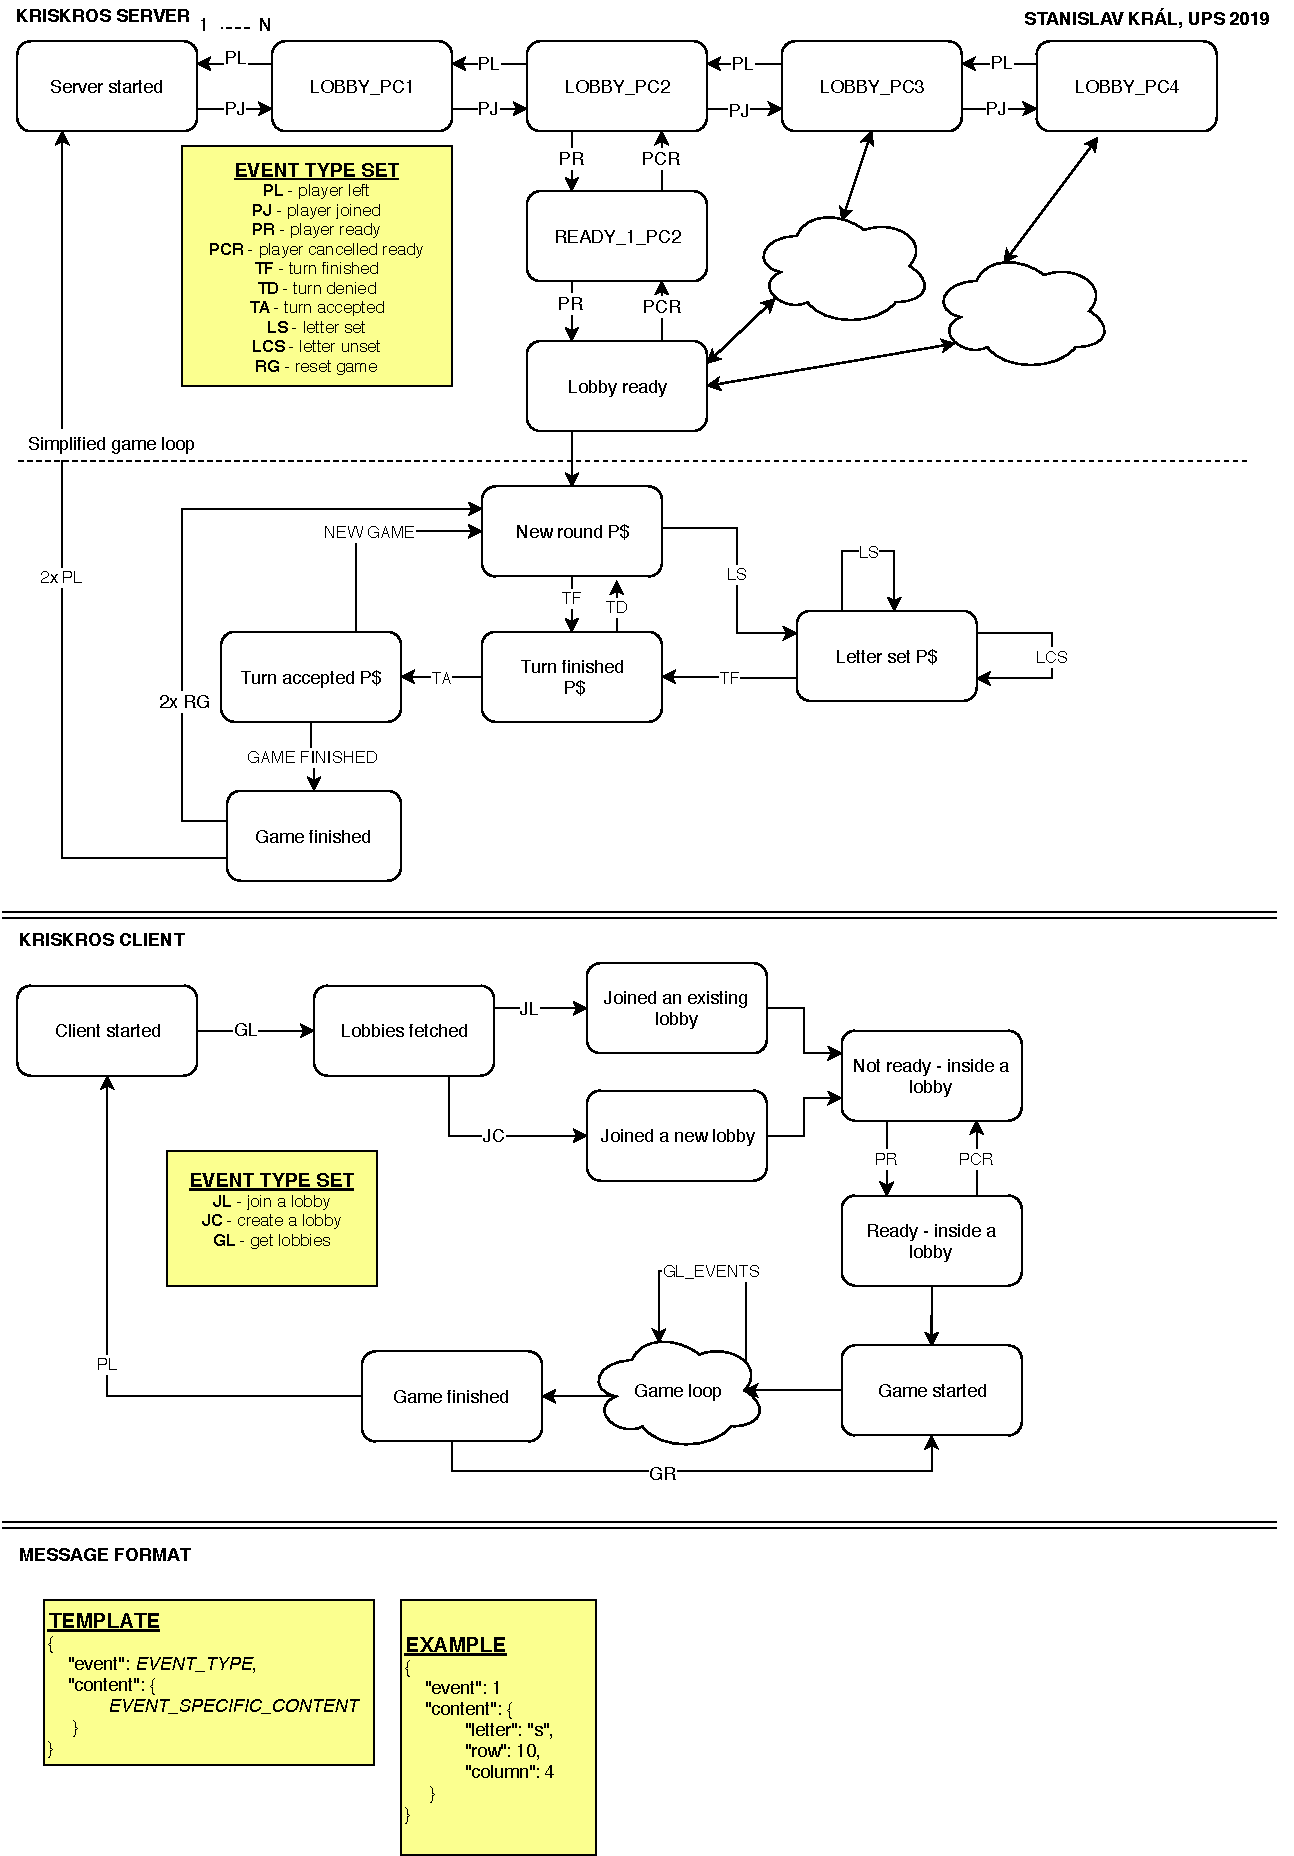
\includegraphics[width=12cm]{img/ups_diagram.png}}
\caption{Zjednodušené UML aplikace (pouze balíčky)}
\label{fig:photo}
\end{figure}
		    \subsubsection{Struktura modulů}

	    \subsection{Popis klienta}
   		    \subsubsection{Struktura modulů}
    
    \section{Závěr}
    


%obrazek
%\begin{figure}[!ht]
%\centering
%{\includegraphics[width=12cm]{img/poly-example.jpeg}}
%\caption{Zjednodušené UML aplikace (pouze balíčky)}
%\label{fig:photo}
%\end{figure}

	
	

\end{document}    